\title{Lecture 11: Random Variable}

\frame{\titlepage}

%%%%%%%%%%%%%
\section[Variable]{Random Variables}
\frame{\sectionpage}
%%%%%%%%%%%%%

\begin{frame}
\frametitle{Warm up}
Recall the formula
\[ P(A) = \frac{n(A)}{n(S)}.\]
This works if all outcomes are \underline{equally likely}. What if they are not?
\end{frame}

\begin{frame}
\frametitle{Two coins}
\addfig{0.8}{two_coins}{Tossing two coins}{}
\end{frame}

\begin{frame}
\frametitle{Catan}
\addfig{0.8}{prob_catan}{\href{https://boardgamegeek.com/boardgame/13/catan}{The Settlers of Catan!}}{}
\end{frame}

\begin{frame}
\frametitle{Variable}
Here are the familiar \textbf{variables}: \pa
\begin{eq*}
3x -4 &=& 5 \pa \\
x^2 + y^2 &=& z^2 \pa \\
x^n + y^n &=& z^n \pa \\
A \cup B &=& \{1,2,4,5\}
\end{eq*}
\end{frame}


\begin{frame}
\frametitle{Random variable}
\begin{defn}{}{}
A \textbf{random variable}, often denoted $X$, describes the outcomes of a statistical experiment in words.
\end{defn} \pa

\begin{ex}
\begin{itemize}
\item Let $X$ = the number of heads you get when you toss 3 fair coins. \pa
\item Let $X$ = the sum of dice values when you roll 4 dice. \pa
\item Let $X$ = the temperature in Munich, Germany tomorrow. \pa
\item Let $X$ = the number of points you get in this class at the end of the semester.
\end{itemize}
\end{ex}
\end{frame}

\iffalse
\begin{frame}
\frametitle{Collaborative Exercise: 1/2}
\begin{itemize}
\item Every one tosses a coin 10 times and record the number of heads.
\item After all members of the class have completed the experiment, announce the result to fill in the table.
\item Let $X$ = the number of heads in ten tosses of the coin.
\end{itemize}
\end{frame}

\begin{frame}
\frametitle{Collaborative Exercise: 2/2}
Answer the questions:
\begin{enumerate}
\item Which value(s) of $x$ occurred most frequently?
\item If you tossed the coin 1,000 times, what values could $x$ take one? Which value(s) of $x$ do you think would occur most frequently?
\item What does the relative frequency column sum to?
\end{enumerate}
\end{frame} 
\fi

\begin{frame}
\frametitle{Notes}
\begin{remark}{}
\begin{itemize}
\item It is not always true that $X$ is in the sample space. For example, the sample space of two coin flips is $\{HH, HT, TH, TT\}$, but if $X$ is the number of heads, then $X=0,1$ or $2$.
\item The random variable $X$ itself doesn't describe an event. Thus, the notation
\[P(X)\]
is meaningless. 
\item We can consider the probability that an outcome takes on certain values. For example, $P(X=1)$ reads ``the probability that $X$ is equal to 1''.
\end{itemize}
\end{remark}
\end{frame}


\begin{frame}
\frametitle{Types of random variables}
There are two different types of random variables: \pa
\begin{defn}{}{}
\begin{itemize}
\item \green{Discrete random variable}: you can list all outcomes separately (e.g. dice, coin, card.) \pa
\item \blue{Continuous random variable}: you can only list outcomes as an interval (e.g. temperature, height, area. Usually those with decimals.) \pa
\end{itemize}
\end{defn}
In this lecture, we are going to focus on \underline{discrete random variables} \pa
\end{frame}

\iffalse
\begin{frame}
\begin{exercisebox}
For each random variable, list all possible values of $X$.
\begin{itemize}
 \item $X = $ the number of heads when you toss 10 fair coins.
 \item $X = $ the difference of two dice.
 \item $X = $ the number of pairs of cards (cards with the same value) when you draw 5 cards from a single standard deck.
 \item $X = $ the temperature of water in Celcius.
\end{itemize}
\end{exercisebox}
\end{frame}
\fi

%%%%%%%%%%%%%
\section[PDF]{Probability Distribution Function}
\frame{\sectionpage}
%%%%%%%%%%%%%

\begin{frame}
\frametitle{Motivation}
\begin{remark}{}
\begin{itemize}
\item Denote the probability that an outcome takes on the value $k$ as $P(X=k)$, or $P(k)$ in short.
\item Since we can find $P(X = k)$ for all possible values $k$, then it is helpful to plot a graph of $k$ versus $P(k)$

\item Such graph is called a \red{function}
\end{itemize}
\end{remark}
\end{frame}

\begin{frame}
\frametitle{Probability Distribution Function (PDF)}
\begin{defn}{}{}
A discrete \textbf{probability distribution function} has two characteristics:
\begin{enumerate}
\item Each probability is between zero and one, inclusive.
\item The sum of the probabilities is 1.
\end{enumerate}
\end{defn}
\end{frame}


\begin{frame}[t]
\begin{ex}
Let $X$ be the value of a single die roll. \pa
\begin{enumerate}
\item For all possible values $k$, find $P(X=k)$
\item Find (a) $P(X=1)$ (b) $P(X\geq 5)$ (c) $P(X \text{ is an odd number})$
\end{enumerate}
\end{ex}
\begin{sol}
\begin{table}[h!]
\begin{tabular}{c |c || c | c| c| c| c | c}
Outcome     & $x$    & 1 & 2  & 3   & 4    & 5    & 6   \\
\hline
Probability &$ P(X=x)$ & $\frac{1}{6}$ & $\frac{1}{6}$ & $\frac{1}{6}$ & $\frac{1}{6}$ & $\frac{1}{6}$ & $\frac{1}{6}$ 
\end{tabular}
\end{table}
\pa 
\begin{itemize}
\item $P(X=1) \pa = \frac{1}{6}$ \pa
\item $P(X \geq 5) \pa = P(5) + P(6) \pa = \frac{2}{6}$ \pa
\item $P(X \text{ is an odd number}) \pa = P(1) + P(3) + P(5) \pa = \frac{3}{6}$ \pa
\end{itemize}
\end{sol}
\end{frame}


\begin{frame}[t]
\begin{ex}
Let $Y$ be the sum of values when rolling two dice. \pause
\begin{enumerate}
\item For all possible values $k$, find $P(Y=k)$
\item Find (a) $P(Y=3)$ (b) $P(Y \leq 4)$ (c) $P(Y \text{ is a square})$
\end{enumerate}
\end{ex}
\begin{sol}
First, list out all $6 \times 6 = 36$ possible outcomes.
\begin{table}[h!]
\renewcommand{\arraystretch}{1.2}
\begin{tabular}{c||c|c|c|c|c|c}
Y & 1 & 2 & 3 & 4  & 5  & 6  \\
\hline
\hline
1                                & 2 & 3 & 4 & 5  & 6  & 7  \\
\hline
2                                & 3 & 4 & 5 & 6  & 7  & 8  \\
\hline
3                                & 4 & 5 & 6 & 7  & 8  & 9  \\
\hline
4                                & 5 & 6 & 7 & 8  & 9  & 10 \\
\hline
5                                & 6 & 7 & 8 & 9  & 10 & 11 \\
\hline
6                                & 7 & 8 & 9 & 10 & 11 & 12
\end{tabular}
\end{table}
\end{sol}
\end{frame}


\begin{frame}
\begin{sol}
Then, we can find the probabilities of each outcome as follows.
\begin{table}[h!]
\begin{tabular}{c || c | c| c| c| c | c|c|c|c|c|c}
$x$    & 2  & 3   & 4    & 5    & 6 & 7 & 8 & 9 & 10 & 11 & 12 \pa  \\
\hline
$ P(Y=x)$ & $\tfrac{1}{36}$ & $\tfrac{2}{36}$ & $\tfrac{3}{36}$ & $\tfrac{4}{36}$ & $\tfrac{5}{36}$ & $\tfrac{6}{36}$  & $\tfrac{5}{36}$ & $\tfrac{4}{36}$ & $\tfrac{3}{36}$ & $\tfrac{2}{36}$ & $\tfrac{1}{36}$ 
\end{tabular}
\end{table} \pa
Thus, we have. \pa
 \begin{eqnarray*}
 P(Y=3) \pa &= &\frac{2}{36} \\ \pause
 P(Y \leq 4) \pa &=& P(2) + P(3) + P(4) \pa = \frac{1}{36} + \frac{2}{36} + \frac{3}{36} \pa = \frac{6}{36}\\ \pa
 P(Y \text{ is a square}) \pa &=& P(4) + P(9) \pa = \frac{7}{36}
 \end{eqnarray*}
 \end{sol}
\end{frame}

\iffalse
\begin{frame}
\begin{table}[h!]
\begin{tabular}{c || c | c| c| c| c | c|c|c|c|c|c}
$k$    & 2  & 3   & 4    & 5    & 6 & 7 & 8 & 9 & 10 & 11 & 12 \pa  \\
\hline
$ P(Y=k)$ & $\frac{1}{36}$ & $\frac{2}{36}$ & $\frac{3}{36}$ & $\frac{4}{36}$ & $\frac{5}{36}$ & $\frac{6}{36}$  & $\frac{5}{36}$ & $\frac{4}{36}$ & $\frac{3}{36}$ & $\frac{2}{36}$ & $\frac{1}{36}$ 
\end{tabular}
\end{table} \pa

\begin{exercise}
Compute the following
 \begin{itemize}
 \item $P(Y = 7)$
 \item $P(Y \geq 8)$
\item $P(Y \mbox{ is even})$
\item $P(Y \mbox{ is divisible by 3})$
 \end{itemize}
 \end{exercise}
\end{frame}
\fi

%%%%%%%%%%%%%
\section[Expected]{Expected Value}
\frame{\sectionpage}
%%%%%%%%%%%%%

\begin{frame}
\frametitle{Motivation}
\begin{itemize}
\item This is where probability meets statistics! \pa
\item $P(X=k)$ only tells you the probability of a single event. \pa
\item What if we want to know what would happen in \blue{long-term}? \pa
\item Or when we repeat the experiments gazillions number of times?
\end{itemize}
\addfig{0.4}{expected_value}{Average?}{}
\end{frame}

% Expected values
\begin{frame}
\frametitle{Expected value $E(X)$}
\begin{defn}{}{}
The \textbf{expected value} (or \textbf{expectation}) \pa of a discrete random variable $X$ is \blue{the "long-term" average} or \blue{mean} of the probability distribution. Formally,
\[ \mu = E(X) = \sum_{x \in S} x P(x)\] \pa
\end{defn}
This means that over the long term of doing an experiment over and over, you would expect this average.
\end{frame}


\begin{frame}[t]
\begin{ex}
Find the expected value of a single die roll. In other words, find $E(X)$ where $X$ is the value of a die roll.
\end{ex}
\begin{sol}
It is helpful to make a table for $P(x)$ and then $x P(x)$.
\begin{table}[h!]
\begin{tblr}{colspec={|Q||Q|Q|Q|Q|Q|Q}, cells={$,c}}
x    & 1 & 2  & 3   & 4    & 5    & 6   \\
 P(x) & \frac{1}{6} & \frac{1}{6} & \frac{1}{6} & \frac{1}{6} & \frac{1}{6} & \frac{1}{6} \\
x P(x) & \frac{1}{6} & \frac{2}{6} & \frac{3}{6} & \frac{4}{6} & \frac{5}{6} & \frac{6}{6} 
\end{tblr}
\end{table}

Then, the expected value of $X$ is 
\[E(X) \pa= \frac{1}{6} + \frac{2}{6} + \frac{3}{6} + \frac{4}{6} + \frac{5}{6} + \frac{6}{6} \pa = \frac{21}{6} \pa = 3.5\]
This means \textit{on average}, the result of a die roll is 3.5 (even though the number is not on the die!). \pa
\end{sol}
\end{frame}


\begin{frame}[t]
\begin{ex}
Find the expected value of a single roll of an 10-sided dice.
\end{ex}
\begin{sol}
It is helpful to make a table for $P(x)$ and then $x P(x)$.
\begin{table}[]
\begin{tblr}{colspec={|Q||Q|Q|Q|Q|Q|Q|Q|Q|Q|Q|}, hlines, cells = {$, c}}
x &1&2&3&4&5&6&7&8&9&10 \\
P(x) & \frac{1}{10} & \frac{1}{10} & \frac{1}{10} & \frac{1}{10} & \frac{1}{10} & \frac{1}{10} & \frac{1}{10}& \frac{1}{10}& \frac{1}{10}& \frac{1}{10} \\
x P(x) & \frac{1}{10} & \frac{2}{10} & \frac{3}{10} & \frac{4}{10} & \frac{5}{10} & \frac{6}{10} & \frac{7}{10}& \frac{8}{10}& \frac{9}{10}& \frac{10}{10}\\
\end{tblr}
\end{table}

Then, the expected value of $X$ is 
\[E(X) \pa= \frac{1}{10} + \frac{2}{10} + \frac{3}{10} + \cdots + \frac{10}{10} \pa = \frac{55}{10} \pa = 5.5\]
This means \textit{on average}, the result of a 10-sided die roll is 5.5.
\end{sol}
\end{frame}


\begin{frame}[t]
\begin{ex}
Find the expected value of the sum of values of \blue{two} dice rolls. In other words, find $E(X)$ where $X$ is the sum of values of two dice rolls.
\end{ex}
\begin{sol}
Make a table for $P(x)$ and then $xP(x)$.
\begin{table}[h!]
\begin{tblr}{colspec={|Q||Q|Q|Q|Q|Q|Q|Q|Q|Q|Q|Q|}, hlines, cells={$,c}}
x&2&3&4&5& 6 & 7 & 8 & 9 & 10 & 11 & 12  \\
P(x) & \tfrac{1}{36} & \tfrac{2}{36} & \tfrac{3}{36} & \tfrac{4}{36} & \tfrac{5}{36} & \tfrac{6}{36} & \tfrac{5}{36} & \tfrac{4}{36} & \tfrac{3}{36} & \tfrac{2}{36} & \tfrac{1}{36}  \\
x P(x) & \tfrac{2}{36} & \tfrac{6}{36} & \tfrac{12}{36} & \tfrac{20}{36} & \tfrac{30}{36} & \tfrac{42}{36} & \tfrac{40}{36} & \tfrac{36}{36} & \tfrac{30}{36} & \tfrac{22}{36} & \tfrac{12}{36}
\end{tblr}
\end{table}
Then, the expected value of $X$ is 
\[E(X) = (2)\frac{1}{36} + (3)\frac{2}{36} + (4)\frac{3}{36} + \ldots + (12)\frac{1}{36} = 7.\]

This means \textit{on average}, the sum of two dice rolls is 7. This agrees with the distribution function that $7$ is the most likely outcome  with probability $\frac{6}{36}$.
\end{sol}
\end{frame}


\begin{frame}[t]
\begin{ex}
Suppose a box contains \red{3 red balls} and \green{5 green balls}. Find the expected number of red balls if you take 3 balls without replacement.
\end{ex}
\begin{sol}
Let $X$ be the number of red balls when taking three balls without replacement. We need to find $P(X = x)$ for $x = 0,1,2$ and $3$. 
\begin{itemize}
\item To get $0$ \red{red balls}, you need to take 3 \green{green balls}. The number of ways to take 3 green balls out of 5 green balls is $\ch{5}{3} = 10$.
\item To get $1$ \red{red ball}, you need to also take 2 \green{green balls}. The number of such ways is $\ch{3}{1} \times \ch{5}{2} = 30$
\item To get $2$ \red{red balls}, you need to also take 1 \green{green ball}. The number of such ways is $\ch{3}{2} \times \ch{5}{1} = 15$.
\item To get all $3$ \red{red balls}, there is only 1 way to do so.
\end{itemize}
\end{sol}
\end{frame}

\begin{frame}[t]
\begin{sol} (continued)
We can verify that we cover all possible outcomes because $10+30+15+1 = 56$, which is equal to the number of ways to take $3$ balls from $8$ balls, or $\ch{8}{3}$.

We now have the following table for $P(x)$ and $xP(x)$
\begin{table}[h!]
\begin{tblr}{colspec={|Q||Q|Q|Q|Q|}, hlines, cells={$,c}}
x & 0 & 1 & 2 & 3 \\
P(x) & \frac{10}{56} & \frac{30}{56} & \frac{15}{56} & \frac{1}{56} \\
xP(x) & 0 & \frac{30}{56} & \frac{30}{56} & \frac{3}{56}
\end{tblr}
\end{table}
Therefore, the expected number of red balls is 
\[ E(X) = 0 + \frac{30}{56} + \frac{30}{56} + \frac{3}{56} = \frac{66}{56} \approx 1.18\]
\end{sol}
\end{frame}


\begin{frame}
\frametitle{Properties of Expected Value}
Notice that rolling two dice gives a total of 7 on average, which is equal twice the average of rolling one die. This is by no mean a coincident!
\begin{thm}{Linearity by sum}{}
Given a random variable $X$ and $Y$. Define $X + Y$ to be a new random variable defined by adding outcomes of $X$ and $Y$. Then, we have
\[E(X+Y) = E(X) + E(Y)\]
\end{thm}
\end{frame}


\begin{frame}[t]
\begin{ex}
Let $X_6$ be the outcome of a single six-sided die roll (abbreviated as \red{d6}), $X_{10}$ be the outcome of a single ten-sided die roll (abbreviated as \blue{d10}).
\begin{enumerate}
\item Find the expected value of totals of one \red{d6} and one \blue{d10}
\item Find the expected value of totals of three \blue{d10}.
\end{enumerate}
\end{ex}
\begin{sol}
\begin{itemize}
\item The expected value of rolling one \red{d6} and one \blue{d10} is \pa
\[E(X_6 +X_{10}) \pa = E(X_6) + E(X_{10}) \pa = 3.5 + 5.5 = 9\]
\item The expected value of rolling three \blue{d10} is
\[E(X_{10} + X_{10} + X_{10}) = E(X_{10}) + E(X_{10}) + E(X_{10}) = 5.5 + 5.5 + 5.5 = 16.5\]
\end{itemize}
\end{sol}
\end{frame}

\begin{frame}
\frametitle{Properties of Expected Value}
Similarly, we have the following property.
\begin{thm}{Linearity by scalar multiplication}{}
Given a random variable $X$ and a constant $a$. Define $aX$ to be a new random variable defined by multiplying $a$ to all outcomes of $X$. Then, we have
\[E(aX) = aE(X)\]
\end{thm}
Note: \red{$2X \neq X+X$} !!! For example, $X$ is the result of a die roll, then possible values of $2X$ are $2,4,6,8,10$ and $12$, which is different from $X+X$ where values range from $2$ up to $12$.
\end{frame}

\begin{frame}
These formula are very useful in answering these types of questions: \pa
\begin{itemize}
\item What gives you a higher sum: rolling 4 \red{d6} or 1 \red{d6} and 2 \blue{d10}? \pa
\item Should I place my settlement around 11,5,9 combinations or 2,6,8 combinations? \pa
\item In a game of Black Jack, I have a 15 hand now. Should I stay or get another card? \pa
\end{itemize}
Informally, you want a \textbf{better payoff}.
\end{frame}


\begin{frame}[t]
\begin{ex}
Suppose you roll 2 dice and gain coins equal to the difference. What is the expected number of coins you would gain?
\end{ex}
\begin{sol}
Let $X$ be the number of coins.
\begin{itemize}
\item $X=0$ when both dice have the same value, which has probability $\frac{6}{36}$
\item $X=1$ when the dice are $(1,2), (2,3), (3,4), (4,5), (5,6), (2,1), (3,2) , (4,3), (5,4), (6,5)$, thus the probability is $\frac{10}{36}$
\end{itemize}
After carefully counting all cases, we have
\[E(X) = (0) \frac{6}{36} + (1) \frac{10}{36} + (2) \frac{8}{36} + (3) \frac{6}{36} + (4) \frac{4}{36} + (5) \frac{2}{36} = \frac{70}{36}\]
\end{sol}
\end{frame}

\iffalse
\begin{frame}
\begin{exercise}
Find the expected number of the following random variables.
 \begin{itemize}
\item $X=$ the face value of a playing card. We consider J, Q and K to have value of zero.
\item $X=$ the number of red marbles drawn from a bag with 8 white marbles and 2 red marbles.
\item $X=$ the sum of rolling a d6, d8, and d10.
\item $X=$ the higher dice when you roll two six-sided dice.
\end{itemize}
 \end{exercise}
\end{frame}
\fi



%%%%%%%%%%%%%
\section[Prob Dist Func]{Probability Distribution Function}
\frame{\sectionpage}
%%%%%%%%%%%%%

\begin{frame}
\frametitle{Questions}
 These are several questions you want to ask:
\begin{tasks}[label = $\circ$]
\task How many \blue{legendary} cards would I get on average if I open 10 packs?
\task If I want to keep buying packs until I get a \blue{legendary} card, how many packs would I need to buy on average? (i.e. how screwed am I?)
\task If I know that a carton of 100 packs has exactly 5 packs with a \blue{legendary} card, how many \blue{legendary} cards would I get if I take 20 packs? 
\task If I know that each carton of 100 packs has various numbers of legendary cards, with the average of 6 cards, how many \blue{legendary} cards would I get if I buy 10 cartons?
\end{tasks}
We will find out in this lecture!
\end{frame}

\begin{frame}
\frametitle{But Why?}
\begin{tasks}[label = $\circ$]
\task If you recognize that your experiment is one of these basic experiments, then you can get all the formulas without having to derive one.
\task If not, then you can first try to simulate your experiment and see if the outcome looks similar to one of these basic experiments.
\task If not, then you will be able to compare your experiments to these basic experiments and see if their tricks can be applied to yours.
\end{tasks}
\end{frame}

\begin{frame}
\frametitle{Probability Distribution Function}
\begin{defn}{}{}
A discrete \textbf{probability distribution function} (or PDF) is a function $P$ of random variable $X$ such that:
\begin{tasks}[label = $\circ$]
\task Each probability is between zero and one, inclusive. In other words, $0 \leq P(x) \leq 1$ for all $x$ in the sample space.
\task The sum of probabilities of all possible values is one. Mathematically writing, $\sum\limits_{x \in S} P(x) = 1$, where $S$ is the sample space (i.e. the set of all possible outcomes).
\end{tasks}
\end{defn}
\end{frame}

\begin{frame}
\begin{ex}
Which function is a probability distribution function?
\end{ex}
\begin{table}
\begin{tabular}{C|C|C|C}
x & 1 & 2 & 3 \\
\hline
P(x) & 0.1 & 0.3 & 1.2
\end{tabular} 
\end{table}

\begin{table}
\begin{tabular}{C|C|C|C}
x & 1 & 2 & 3 \\
\hline
P(x) & 0.1 & 0.3 & 0.5
\end{tabular} 
\end{table}

\begin{table}
\begin{tabular}{C|C|C|C}
x & 1 & 2 & 3 \\
\hline
P(x) & 0.2 & 0.5 & 0.3
\end{tabular} 
\end{table}
\end{frame}

\begin{frame}
\frametitle{Exercise}
Solution
\begin{table}
\begin{tabular}{C|C|C|C}
x & 1 & 2 & 3 \\
\hline
P(x) & 0.1 & 0.3 & \red{1.2}
\end{tabular} 
\end{table}

\begin{table}
\begin{tabular}{C|C|C|C}
x & 1 & 2 & 3 \\
\hline
P(x) & 0.1 & 0.3 & 0.5
\end{tabular} 
\end{table}
\[0.1 + 0.3 + 0.5 = 0.9 \red{\neq 1}\]

\begin{table}
\begin{tabular}{C|C|C|C}
x & 1 & 2 & 3 \\
\hline
P(x) & 0.2 & 0.5 & 0.3
\end{tabular} 
\end{table}
\[0.2 + 0.5 + 0.3 = 1\]
\end{frame}

\begin{frame}
\frametitle{Representation of PDF as a bar chart}
It is useful to represent a probability distribution function as a bar chart where
\begin{tasks}[label = $\circ$]
\task The x-axis represents all outcomes.
\task The y-axis represents the probability of that outcome.
\end{tasks}
\begin{columns}
\begin{column}{0.45\textwidth}
\begin{table}
\begin{tabular}{C|C|C|C}
x & 0 & 1 & 2 \\
\hline
P(x) & \frac{1}{4} & \frac{2}{4} & \frac{1}{4}
\end{tabular} 
\end{table}
\end{column}
\begin{column}{0.45\textwidth}
\begin{figure}[h!]
\centering
\begin{tikzpicture}[yscale = 4]
\draw[->] (0,0) -- (4,0) node [right] {$x$};
\draw[->] (0,0) -- (0,0.6) node [above] {$P(x)$};
\foreach \x / \y in {0/0.25,1/0.5,2/0.25} 
{
	\draw (\x+1, 0) -- (\x+1,-0.1) node [below] {$\x$};
	\draw (\x+0.8, 0) rectangle (\x+1.2, \y);
}
\foreach \x in {0,0.25,0.5}
{
	\draw (-0.1, \x) -- (0, \x) node [left] {$\x$};
}
\node at (2,-1) {Number of heads};
\node[rotate = 90] at (-1, 0.25) {Probability};
\end{tikzpicture}
\end{figure}
\end{column}
\end{columns}
\end{frame}

\begin{frame}
\frametitle{Uniform Distribution}
The most basic distribution is a uniform distribution function.
\begin{defn}{}{}
A \textbf{uniform distribution} is a probability distribution function $P$ such that 
\begin{tasks}[label = $\circ$]
\task The number of possible outcomes (the sample space $S$) is finite.
\task All outcomes are equally likely. In particular, for any outcome $k \in S$, we have $P(X=k) = \frac{1}{n}$ where $n$ is the number of outcomes.
\end{tasks}
\end{defn}
\end{frame}


%%%%%%%%%%%%%
\section{Binomial}
\frame{\sectionpage}
%%%%%%%%%%%%%

\begin{frame}
\frametitle{Motivation}
\begin{block}{} \begin{center}How many \blue{legendary} cards would I get on average if I open 10 packs?\end{center}\end{block}
\begin{figure}[h!]
\includegraphics[width = 0.9\textwidth]{l11i03}
\end{figure}
\end{frame}


\begin{frame}[t]
\begin{ex}
Let $X$ = the number of heads from 3 coin flips. Draw the bar chart of the probability distribution function.
\end{ex}
\begin{sol} 
Compute each $P(X=k)$ separately. For $X=0$, the only way to get 0 heads is when all three coins are tails, and the probability is 
\[P(X=0) = \frac{1}{2} \times \frac{1}{2} \times \frac{1}{2} = \frac{1}{8}.\]

For $X=1$, there are 3 such outcomes - namely HTT, THT, and TTH. Hence, 
\[P(X=1) = 3 \times \frac{1}{8} = \frac{3}{8}.\]

Similary, we can compute $P(X=2) = \frac{3}{8}$ and $P(X=3) = \frac{1}{8}$.
\end{sol}
\end{frame}

\begin{frame}
\begin{sol} (Continued) Thus, we have the following table
\begin{table}[h!]
\def\arraystretch{2}
\begin{tabular}{|C|C|C|C|C|}
\hline
k & 0 & 1 & 2 & 3\\
\hline
P(X=k) & \frac{1}{8} & \frac{3}{8} & \frac{3}{8} & \frac{1}{8}\\
\hline
\end{tabular}
\end{table}

Using the table above, we can make the folowing chart.
\begin{figure}[h!]
\centering
\begin{tikzpicture}
\draw[->] (0,0) -- (5,0) node [right] {$k$};
\draw[->] (0,0) -- (0,2) node [above] {$P(k)$};
\foreach \x / \y in {0/0.125,1/0.375,2/0.375,3/0.125} 
{
	\draw (\x+1, 0) -- (\x+1,-0.1) node [below] {$\x$};
	\draw (\x+0.8, 0) rectangle (\x+1.2, 4*\y);
}
\foreach \x in {1,2,3}
{
	\draw (-0.1, \x/2) -- (0, \x/2) node [left] {$\x/8$};
}
\end{tikzpicture}
\end{figure}
\end{sol}
\end{frame}

\begin{frame}
\frametitle{Binomial Distribution}
\begin{defn}{}{}
A \textbf{binomial experiment} has three characteristics
\begin{tasks}[label = $\circ$]
\task There are a fixed number of $n$ trials.
\task There are only two possible outcomes: success or failure. Let $p$ be the probability of a success on a single trial.
\task All $n$ trials are independent and are repeated using identical condition.
\end{tasks}
\end{defn}

\begin{block}{}
Let $X$ be the number of successes obtained in the $n$ independent trails. Then, $P(X)$ is called a \textbf{a binomial probability distribution}.
\end{block}
\end{frame}


\begin{frame}[t]
\begin{ex}
\begin{tasks}[label = $\circ$]
\task The number of 1s from 10 dice rolls.
\task The number of times you get a blackjack in 100 games.
\task The number of times you win a last-two-digit lottery prize, given that you buy one lottery biweekly 24 times in a row.
\end{tasks}
\end{ex}
\addfig{0.6}{binomial_example}{\href{https://www.youtube.com/watch?v=WR0nMTr6uOo}{Electrifying }}
\end{frame}

\begin{frame}
\frametitle{Example of binomial distributions}
\begin{figure}

\includegraphics[width = 0.6\textwidth]{l11i06}
\caption{\href{https://homepage.divms.uiowa.edu/~mbognar/applets/bin.html}{Click here to try it!}}
\end{figure}
\end{frame}

\begin{frame}
\frametitle{Formulas (1/2)}
\begin{tasks}[label = $\circ$]
\task The probability of exactly $k$ successes in $n$ trials is $$P(X=k) = \ch{n}{k} p^k (1-p)^{n-k}.$$
\task The expected number is $$\mu = E(X) = np.$$
\end{tasks}
\end{frame}

\begin{frame}
\frametitle{Formulas (2/2)}
These are irrelevent to our course, but for the sake of completeness here are other variables.
\begin{tasks}[label = $\circ$]
\task The variance is $$\sigma^2 = V(X) = np(1-p).$$
\task The standard variation is $$\sigma = \sqrt{np(1-p)}.$$
\end{tasks}
\end{frame}

\begin{frame}
\frametitle{Notes}
\begin{tasks}[label = $\circ$]
\task A binomial experiment (or a ``coin flip'') with only one trial $(n=1)$ is called a \textbf{Bernoulli Trial}.
\task We denote $X \sim B(n,p)$, read as $X$ is a random variable with a binomial distribution.
\end{tasks}
\end{frame}

%%%%%%%%%%%%%
\section{Geometric}
\frame{\sectionpage}
%%%%%%%%%%%%%

\begin{frame}
\frametitle{Motivation}
\begin{block}{} \begin{center}If I want to keep buying packs until I get a \blue{legendary} card, how many packs would I need to buy on average? (i.e. how screwed am I?)\end{center}\end{block}
\begin{figure}[h!]

\includegraphics[width =0.9\textwidth]{l11i07}
\end{figure}
\end{frame}


\begin{frame}[t]
\begin{ex}
Let $X$ = the number of flips before you get the first head (i.e. all previous flips are tails). Draw the bar chart of the probability distribution function.
\end{ex}
\begin{sol}
Let's consider each possible value of $X$ one by one. If the first flip is head, then we have $X=0$ as there was no prior failure, and we can see that $P(X=0) = \frac{1}{2}$. Then, for $X=1$, the first flip must be tail, and the second flip must be head. Since the two flips are independent, we have $P(X=1) = \frac{1}{2} \times \frac{1}{2} = \frac{1}{4}$. Similarly, we can easily prove that
\[ P(X=k) = \frac{1}{2} \times \left( \frac{1}{2}\right)^k.\]
\end{sol}
\end{frame}

\begin{frame}
\begin{sol} (Continued) 
Thus, we have the following table
\begin{table}[h!]
\def\arraystretch{2}
\begin{tabular}{|C|C|C|C|C|C|C|}
\hline
k & 0 & 1 & 2 & 3 & 4 & \ldots \\
\hline
P(X=k) & \frac{1}{2} & \frac{1}{4} & \frac{1}{8} & \frac{1}{16} & \frac{1}{32} & \ldots \\
\hline
\end{tabular}
\end{table}

Using the table above, we can make the folowing chart.
\begin{figure}[h!]
\centering
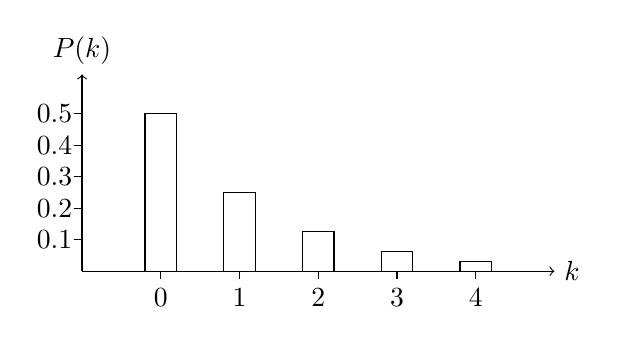
\begin{tikzpicture}
\draw[->] (0,0) -- (6,0) node [right] {$k$};
\draw[->] (0,0) -- (0,2.5) node [above] {$P(k)$};
\foreach \x in {0,1,2,3,4} 
{
	\draw (\x+1, 0) -- (\x+1,-0.1) node [below] {$\x$};
	\draw (\x+0.8, 0) rectangle (\x+1.2, 2*0.5^\x);
}
\foreach \x in {0.1,0.2,0.3,0.4,0.5}
{
	\draw (-0.1, 4*\x) -- (0, 4*\x) node [left] {$\x$};
}
\end{tikzpicture}
\end{figure}
\end{sol}
\end{frame}


\begin{frame}
\frametitle{Geometric Distribution}
\begin{defn}{}{}
A \textbf{geometric experiment} has three characteristics
\begin{tasks}[label = $\circ$]
\task There are one or more Bernoulli trials with \textbf{ALL} failures \textbf{EXCEPT} the last one, which is a success.
\task There must be at least one trial, but in theory the number of trials could go on forever.
\task The probability of a success is the same number $\red{p}$  for each trial.
\end{tasks}
\end{defn}
\end{frame}


\begin{frame}[t]
\begin{block}{}
Let $X$ be the number of independent trials \textbf{before} the first success. Then, $P(X)$ is called a \textbf{a geometric probability distribution}.

We denote $X \sim G(p)$, read as $X$ is a random variable with a geometric distribution.
\end{block}

\begin{ex}
\begin{tasks}[label = $\circ$]
\task The number of lotteries, if you buy one biweekly until you win a last-two-digit prize.
\task The number of friends you have a handshake with until you get a COVID-19.
\task The number of partners you go out with until you find the TRUE LOVE.
\end{tasks}
\end{ex}
\end{frame}

\begin{frame}
\frametitle{Example of geometric distributions}
\begin{figure}

\includegraphics[width = 0.6\textwidth]{l11igeometric}
\caption{\href{https://homepage.divms.uiowa.edu/~mbognar/applets/geo1.html}{Click here to try it!}}
\end{figure}
\end{frame}


\begin{frame}
\frametitle{Formulas}
\begin{tasks}[label = $\circ$]
\task The probability of exactly $k$ failures before the first success is $$P(X=k) = p(1-p)^k.$$
Note that this implies there are $k+1$ trials in total.
\task The expected number is $$\mu = E(X) = \frac{1-p}{p}.$$
\end{tasks}
\end{frame}

\begin{frame}
\frametitle{Formulas}
Again, these are irrelevent to our course, but for the sake of completeness here are other variables.
\begin{tasks}[label = $\circ$]
\task The variance is $$\sigma^2 = V(X) = \frac{1}{p} \left( \frac{1}{p} - 1\right).$$
\task The standard variation is $$\sigma = \sqrt{\frac{1}{p} \left( \frac{1}{p} - 1\right)}.$$
\end{tasks}
\end{frame}


\begin{frame}[t]
\begin{ex}
Suppose that you are performing the probability experiment of rolling one fair six-sided die. Let F be the event of rolling a four or a five. You are interested in how many times you need to roll the die in order to obtain the first four or five as the outcome.
\begin{itemize}
\item $p$ = probability of success (event F occurs)
\item $q$ = probability of failure (event F does not occur)
\end{itemize}
\begin{tasks}(1)
\task Write the description of the random variable $X$.
\task What are the values that $X$ can take on?
\task Find the values of $p$ and $q$.
\task Find the probability that the first occurrence of event F (rolling a four or five) is on the second trial.
\end{tasks}
\end{ex}
\end{frame}

\begin{frame}
\begin{sol}
\begin{tasks}(1)
\task $X =$ the number of dice rolls before the first four or five outcome.
\task $X$ can take on $0,1,2,\ldots$. In other words, any natural number (including 0).
\task $p = \frac{2}{6} = \frac{1}{3}$ and $q = 1-p = 1 - \frac{1}{3} = \frac{2}{3}$
\task We can compute it directly: to get the success on the second trial, the first trial needs to be a failure. Therefore, $P(X=1) = \frac{2}{3} \times \frac{1}{3} = \frac{2}{9}.$

On the other hand, we can apply the formula directly with $k=1$ to get
\[ P(X=1) = p (1-p)^k = \frac{1}{3} \left( \frac{2}{3} \right)^1 = \frac{2}{9}\]
\end{tasks}
\end{sol}
\end{frame}


%%%%%%%%%%%%%
\section{Extra}
\frame{\sectionpage}
%%%%%%%%%%%%%

\begin{frame}
\frametitle{Motivation}
\begin{block}{} \begin{center}If I know that a bundle of 100 packs has exactly 5 packs with a \blue{legendary} card, how many \blue{legendary} cards would I get if I take 20 packs?\end{center}\end{block}
\begin{figure}[h!]

\includegraphics[width = 0.8\textwidth]{l11i08}
\end{figure}
\end{frame}


\begin{frame}
\frametitle{Hypergeometric Distribution}
\begin{defn}{}{}
A \textbf{hypergeometric experiment} has five characteristics
\begin{tasks}[label = $\circ$]
\task You take samples from \textbf{two} groups.
\task You are concerned with a group of interest, called the first group.
\task You sample \textbf{without replacement} from the combined groups.
\task Each pick is \textbf{not} independent.
\task You are \textbf{not} dealing with Bernoulli Trials (due to dependency).
\end{tasks}
\end{defn}
\end{frame}


\begin{frame}
\begin{block}{}
Let $X$ be the number of items from the first group. Then, $P(X)$ is called a \textbf{a hypergeometric probability distribution}.

We denote $X \sim H(r,b,n)$ where $r$ is the size of the first group (the group of interest), $b$ is the size of the second group, and $n$ is the size of the chosen sample.
\end{block}
\begin{ex}
\begin{tasks}[label = $\circ$]
\task The number of boys when you select 10 random people from the class.
\task The number of good apples when buying 5 from a pile of apples.
\task The number of unplayed games on your Steam account when you take 10 random games.
\end{tasks}
\end{ex}
\end{frame}

\begin{frame}
\frametitle{Example of hypergeometric distributions}
\begin{figure}

\includegraphics[width = 0.6\textwidth]{l11hypergeo}
\caption{\href{https://homepage.divms.uiowa.edu/~mbognar/applets/hg.html}{Click here to try it!}}
\end{figure}
\end{frame}

\begin{frame}
\frametitle{Motivation}
\begin{block}{} \begin{center}If I know that each bundle of packs (exact amount doesn't matter) has various numbers of legendary cards, with the average of 5 cards per bundle, how many \blue{legendary} cards would I get if I buy 10 bundles?\end{center}\end{block}
\begin{figure}[h!]

\includegraphics[width = 0.8\textwidth]{l11i09}
\end{figure}
\end{frame}

\begin{frame}
\frametitle{Poisson Distribution}
\begin{defn}{}{}
A \textbf{Poisson experiment} has two characteristics
\begin{tasks}[label = $\circ$]
\task The \textbf{Poisson probability distribution} gives the probability of a number of events occurring in a fixed interval of
time or space if these events happen with a known average rate and independently of the time since the last event.
\task The Poisson distribution may be used to approximate the binomial if the probability of success is ``small" (such as $p=0.01$) and the number of trials is ``large" (such as $n=1,000$). 
\end{tasks}

\end{defn}
\end{frame}


\begin{frame}
\begin{block}{}
We denote $X \sim P(\mu)$, read as $X$ is a random variable with a Poisson distribution. The parameter is $\mu$ which is the mean for the interval of interest.
\end{block}
\begin{ex}
\begin{tasks}[label = $\circ$]
\task The number of pieces of mail received in a day.
\task The number of phone calls received by a call center per hour.
\task The number of fake COVID-19 news on your facebook feed in an hour.
\end{tasks}
\end{ex}
\end{frame}

\begin{frame}
\frametitle{Example of Poisson Distribution}
\begin{figure}

\includegraphics[width = 0.6\textwidth]{l11poisson}
\caption{\href{https://homepage.divms.uiowa.edu/~mbognar/applets/bin-like.html}{Click here to try it!}}
\end{figure}
\end{frame}
